% Options for packages loaded elsewhere
\PassOptionsToPackage{unicode}{hyperref}
\PassOptionsToPackage{hyphens}{url}
%
\documentclass[
  english,
  man]{apa6}
\usepackage{lmodern}
\usepackage{amssymb,amsmath}
\usepackage{ifxetex,ifluatex}
\ifnum 0\ifxetex 1\fi\ifluatex 1\fi=0 % if pdftex
  \usepackage[T1]{fontenc}
  \usepackage[utf8]{inputenc}
  \usepackage{textcomp} % provide euro and other symbols
\else % if luatex or xetex
  \usepackage{unicode-math}
  \defaultfontfeatures{Scale=MatchLowercase}
  \defaultfontfeatures[\rmfamily]{Ligatures=TeX,Scale=1}
\fi
% Use upquote if available, for straight quotes in verbatim environments
\IfFileExists{upquote.sty}{\usepackage{upquote}}{}
\IfFileExists{microtype.sty}{% use microtype if available
  \usepackage[]{microtype}
  \UseMicrotypeSet[protrusion]{basicmath} % disable protrusion for tt fonts
}{}
\makeatletter
\@ifundefined{KOMAClassName}{% if non-KOMA class
  \IfFileExists{parskip.sty}{%
    \usepackage{parskip}
  }{% else
    \setlength{\parindent}{0pt}
    \setlength{\parskip}{6pt plus 2pt minus 1pt}}
}{% if KOMA class
  \KOMAoptions{parskip=half}}
\makeatother
\usepackage{xcolor}
\IfFileExists{xurl.sty}{\usepackage{xurl}}{} % add URL line breaks if available
\IfFileExists{bookmark.sty}{\usepackage{bookmark}}{\usepackage{hyperref}}
\hypersetup{
  pdftitle={Exploring Anomalies in Pacific Northwest Special Education Trends},
  pdfauthor={David Fainstein1, Janette Avelar1, Makayla Whitney1, \& Joe Swinehart1},
  pdflang={en-EN},
  pdfkeywords={Vancouver, British Columbia, Oregon, Special Education, SpEd},
  hidelinks,
  pdfcreator={LaTeX via pandoc}}
\urlstyle{same} % disable monospaced font for URLs
\usepackage{graphicx,grffile}
\makeatletter
\def\maxwidth{\ifdim\Gin@nat@width>\linewidth\linewidth\else\Gin@nat@width\fi}
\def\maxheight{\ifdim\Gin@nat@height>\textheight\textheight\else\Gin@nat@height\fi}
\makeatother
% Scale images if necessary, so that they will not overflow the page
% margins by default, and it is still possible to overwrite the defaults
% using explicit options in \includegraphics[width, height, ...]{}
\setkeys{Gin}{width=\maxwidth,height=\maxheight,keepaspectratio}
% Set default figure placement to htbp
\makeatletter
\def\fps@figure{htbp}
\makeatother
\setlength{\emergencystretch}{3em} % prevent overfull lines
\providecommand{\tightlist}{%
  \setlength{\itemsep}{0pt}\setlength{\parskip}{0pt}}
\setcounter{secnumdepth}{-\maxdimen} % remove section numbering
% Make \paragraph and \subparagraph free-standing
\ifx\paragraph\undefined\else
  \let\oldparagraph\paragraph
  \renewcommand{\paragraph}[1]{\oldparagraph{#1}\mbox{}}
\fi
\ifx\subparagraph\undefined\else
  \let\oldsubparagraph\subparagraph
  \renewcommand{\subparagraph}[1]{\oldsubparagraph{#1}\mbox{}}
\fi
% Manuscript styling
\usepackage{upgreek}
\captionsetup{font=singlespacing,justification=justified}

% Table formatting
\usepackage{longtable}
\usepackage{lscape}
% \usepackage[counterclockwise]{rotating}   % Landscape page setup for large tables
\usepackage{multirow}		% Table styling
\usepackage{tabularx}		% Control Column width
\usepackage[flushleft]{threeparttable}	% Allows for three part tables with a specified notes section
\usepackage{threeparttablex}            % Lets threeparttable work with longtable

% Create new environments so endfloat can handle them
% \newenvironment{ltable}
%   {\begin{landscape}\begin{center}\begin{threeparttable}}
%   {\end{threeparttable}\end{center}\end{landscape}}
\newenvironment{lltable}{\begin{landscape}\begin{center}\begin{ThreePartTable}}{\end{ThreePartTable}\end{center}\end{landscape}}

% Enables adjusting longtable caption width to table width
% Solution found at http://golatex.de/longtable-mit-caption-so-breit-wie-die-tabelle-t15767.html
\makeatletter
\newcommand\LastLTentrywidth{1em}
\newlength\longtablewidth
\setlength{\longtablewidth}{1in}
\newcommand{\getlongtablewidth}{\begingroup \ifcsname LT@\roman{LT@tables}\endcsname \global\longtablewidth=0pt \renewcommand{\LT@entry}[2]{\global\advance\longtablewidth by ##2\relax\gdef\LastLTentrywidth{##2}}\@nameuse{LT@\roman{LT@tables}} \fi \endgroup}

% \setlength{\parindent}{0.5in}
% \setlength{\parskip}{0pt plus 0pt minus 0pt}

% \usepackage{etoolbox}
\makeatletter
\patchcmd{\HyOrg@maketitle}
  {\section{\normalfont\normalsize\abstractname}}
  {\section*{\normalfont\normalsize\abstractname}}
  {}{\typeout{Failed to patch abstract.}}
\patchcmd{\HyOrg@maketitle}
  {\section{\protect\normalfont{\@title}}}
  {\section*{\protect\normalfont{\@title}}}
  {}{\typeout{Failed to patch title.}}
\makeatother
\shorttitle{PACNW SpEd Trends}
\keywords{Vancouver, British Columbia, Oregon, Special Education, SpEd\newline\indent Word count: 0<n<1,000,000}
\DeclareDelayedFloatFlavor{ThreePartTable}{table}
\DeclareDelayedFloatFlavor{lltable}{table}
\DeclareDelayedFloatFlavor*{longtable}{table}
\makeatletter
\renewcommand{\efloat@iwrite}[1]{\immediate\expandafter\protected@write\csname efloat@post#1\endcsname{}}
\makeatother
\usepackage{csquotes}
\ifxetex
  % Load polyglossia as late as possible: uses bidi with RTL langages (e.g. Hebrew, Arabic)
  \usepackage{polyglossia}
  \setmainlanguage[]{english}
\else
  \usepackage[shorthands=off,main=english]{babel}
\fi

\title{Exploring Anomalies in Pacific Northwest Special Education Trends}
\author{David Fainstein\textsuperscript{1}, Janette Avelar\textsuperscript{1}, Makayla Whitney\textsuperscript{1}, \& Joe Swinehart\textsuperscript{1}}
\date{}


\authornote{

Janette Avelar, University of Oregon College of Education

David Fainstein, University of Oregon College of Education

Joe Swinehart, Behavioral Research \& Teaching

Makayla Whitney, University of Oregon College of Education

Project completed using RStudio, GitKraken, GitHub, and papaja

Contact: \href{mailto:dfainste@uoregon.edu}{\nolinkurl{dfainste@uoregon.edu}}

The authors made the following contributions. David Fainstein: Conceptualization, Writing - Original Draft Preparation, Writing - Review \& Editing; Janette Avelar: Writing - Review \& Editing; Makayla Whitney: Writing - Review \& Editing; Joe Swinehart: Writing - Review \& Editing.

Correspondence concerning this article should be addressed to David Fainstein, 1655 Alder, Eugene, Oregon, USA 97403. E-mail: \href{mailto:dfainste@uoregon.edu}{\nolinkurl{dfainste@uoregon.edu}}

}

\affiliation{\vspace{0.5cm}\textsuperscript{1} University of Oregon}

\abstract{
This paper will examine the changes in public school special education populations in Vancouver, British Columbia and Oregon over the last 20 years. The British Columbia (BC) data was pulled from an open-source data catalogue, published by the education analytics division of the Ministry of Education in British Columbia. This longitudinal data acquistion is part of formal student status reporting that is required within BC public schools - typically occuring in October of each school year. The Oregon data was pulled from the Oregon Department of Education and covers special education enrollment from 2002 - 2020. This data acquistion is part of formal student status reporting that is required for compliance with federal IDEA laws - typically occuring in November or February of each school year. Within the BC dataset, students with exceptionalities are categorized in one of 12 eligibility categories; within the Oregon dataset, this is 13 categories.
}



\begin{document}
\maketitle

\hypertarget{introduction}{%
\section{Introduction}\label{introduction}}

Educational policy can impact practice by reorganizing educational delivery and reconceptualizing the meaning and impact of education on society (Ball, 1998). Educational policy exists as a mechanism to drive changes in school buildings that result in socially important outcomes (e.g., increasing literacy acquisition through improved instruction, reducing instances of bullying through prevention programs). However, the relationship between policy and practice in Western formal systems of education is often unclear, misdirected, or atheoretical (Cohen et al., 2009). Leveraging the power of policy as a change agent for the delivery and conceptualization of education stands to benefit a significant proportion of students (Swanson, 2007).

When policy is enacted, the intended outcomes are often not realized for months, years, or decades (Gu et al., 2018). For example, changing school district policy on professional development to align with research-informed practices may be constructed to increase student academic achievement; though, there is insufficient evidence pointing to how long professionalized intervention with teachers will take to increase student academic scores (Luke \& McArdle, 2009). Longitudinal data helps to understand the impact of policy change because of the year-over-year comparisons that illustrate differences, inflection points, or anomalies of interest (Michelmore \& Dynarski, 2017).

\hypertarget{current-study}{%
\subsection{Current Study}\label{current-study}}

Our project primarily examines two datasets detailing head counts of students with exceptionalities eligible for special education services aged 6-21. The datasets offer insights to the categorization for special education eligibility in public schools within British Columbia (BC) and Oregon (OR). The head counts from BC are collected from 2002/2003 to the most recent data from 2019/2020. The OR head counts are drawn from an annual dataset spanning 2002 through 2020. Levels of categorization include school-, district-, and provincial-level head counts for BC. The OR data set includes state-wide head counts that are not aggregated by school or district.

We intend to explore several questions regarding longitudinal trends where educational policy may have impacted special education practice. First, we will use descriptive statistics to describe trends in disability prevalence over time. The initial analyses will inform a discussion on developmental trajectories by illustrating shifts in prevalence growth from static to linearly increasing based on age of diagnosis for the Oregon data, which can serve as a springboard to make inferences about BC data (e.g., common age of onset for diagnosis per category and diagnostic patterns over time). In studying the differences and similarities between OR and BC datasets, we will also engage in a discussion on diagnostic terminology across regions with respect to the definitions as detailed by the Diagnostic and Statistical Manual of Mental Disorders (DSM; American Psychological Association, 2013), in part as a response to a challenge set by differing terminology between BC and OR categorization (i.e., the United States federal guidelines for exceptionality designation are similar but not identical to exceptionality designation guidelines in BC).

Second, we hope to closely analyze any changes, or lack thereof, within the BC data following Canadian Supreme Court rulings between the British Columbia Teachers Federation and the province of BC (See Lambert, 2017). Canadian supreme court rulings have significant implications on educational policy in the provinces and, in 2016, resulted in a limit to the number of students with disability designations in classrooms resulting in an expansion of the number of specialist teachers' that school districts are required to hire. The driving theory of change is that decreasing student-to-teacher ratios and capping the number of students with exceptionalities in each classroom causes student designation practices to change. Theoretically, school district administrators made decisions based on current staffing levels, student designations, diagnostic capacity and malleability, as well as external pressures to adjust practice according to legal mandates.

Finally, we will explore differences between urban and rural school districts in BC. Districts are categorized by population size and proximity to metropolitan areas, as recorded and defined by the Statistics Canada census from 2016. School district level data is useful for examining longitudinal trends for individual administrative units (e.g., superintendent's office and director(s) of inclusive education); however, this level of data analysis cannot speak to province-wide trends in the culture of superordinate legal directives which impact swift policy changes. Given this, we will run analyses on both exemplar districts to highlight localized policy impacts on practice and amalgamated districts (e.g., school districts defined as rural by Statistics Canada) to investigate cultural shifts in the policy-to-practice association.

\hypertarget{problem-statement-and-rqs}{%
\subsection{Problem Statement and RQs}\label{problem-statement-and-rqs}}

In comparison to the United States, Canadian education policy receives little attention and scholarly interest (Walker \& Bergmann, 2013). While Canadian K-12 academic achievement outcomes are generally higher than a national-level comparison with the US, there are ongoing policy issues to address when provincial ministries of education are crafting legislation and procedures to impact a top-tier system of education. Significant events, such as the 2016 Canadian supreme court ruling that directly impacted British Columbia classrooms, have downstream effects on instructional interactions; yet a retroactive policy lens is rarely applied after such events occur. The current study seeks to address the knowledge gap of downstream instructional interact effects after a significant event in BC educational policy.

With respect to the 2016 Supreme Court of Canada decision to revert BC classroom composition, size, and ratios for specialist teachers:
(1) Do student prevalence rates of disability or disorder decrease after the supreme court ruling of 2016 against existing trends?
(2) Are there different patterns for disability or disorder designation for rural versus urban school districts after the supreme court ruling in 2016?

\hypertarget{methods}{%
\section{Methods}\label{methods}}

Datasets were extracted from publicly available sources. Specifically, the BC Ministry of Education, Oregon Department of Education, and Statistics Canada are the data sources for the current study. Note that the primary jurisdiction of interest is BC, and OR is selected as a reasonable basis of comparison (i.e., similar geography, population, and population growth rate). Further, BC has distinct educational policy from OR as Canadian education is administered entirely by provincial ministries of education and special education law is remarkably different between BC and OR. Together, these datasets help achieve three objectives for acquiring data appropriate to the research questions:
Headcount data at multiple levels (e.g., district and state or province) for students with exceptionalities, disaggregated by category of exceptionality, year, and location.
Population data to fit school district locations to a geographical classification (e.g., urban, suburban, rural) as specified in national documentation (e.g., urban centers have a minimum of 10,000 inhabitants based on census data), and calculate prevalence rates.
Data from multiple jurisdictions where educational policies do not align chronologically. For example, special education law in the United States is disjointed from BC special education law and policy changes are not the same, nor are they implemented simultaneously.

The nature of the current study is intentionally exploratory within a systematic approach of viewing data, testing a priori hypotheses against descriptive statistics, calculating effect sizes if appropriate, and, finally, exploring notable anomalies in prevalence trends that were not hypothesized a posteriori. As a first step, the authors took the approach of examining provincial-level data in BC. Then, trends in BC data were compared against trends in OR data to see if similar rates of students were designated with exceptionalities across jurisdictions. When anomalies were suspected in the BC trends of exceptionality prevalence, then effect size tests were conducted in line with the research questions. Finally, any anomalies that were suspected a posteriori were tested with effect size calculations and discussed in the final section of our current study.

The three datasets were used for analysis in R (cite R) for reproducibility and data visualization. All code for analysis and data representation is publicly available for reproducibility (\url{https://github.com/JoeSwinehart/datascienceproject}). There are several caveats for data use and cleaning in the current analysis. First, the BC and OR datasets were not a completely parallel comparison, because the OR data set includes a broader age range of students (ages 3 - 21) as compared to the BC data set (ages 5 - 19). The Oregon data set was pared down to include a similar age range to BC data; however, it is worth noting that differences in age range may represent different approaches to diagnostic categorization (e.g., intellectual disability in BC can be diagnosed at age 5; whereas the Oregon data follows IDEA where it is more likely young children will be categorized as developmentally delayed). Second, data masking necessitates a decision-point for analysis. Specifically, the BC Ministry of Education data masks all cells with headcounts below 10 students, therefore our analyses left out these cases when computing effect sizes for provincial-level data. Data masking was most prominently an issue when examining school district-level data in BC, as smaller school districts often masked low-incidence exceptionality data. When appropriate, masked data is assigned a conservative estimate of (n = 9) such that enough data units were included in effect size comparisons. Third, Canadian census data from 2016 is the basis of classification for district geographical location (e.g., urban, suburban, rural, exurban). Due to the geographical distribution of population in BC, only two categories are used for the current analyses: urban and rural. Fourth, due to low population numbers with independent schools in BC, the current study will only examine public school data for the years 2002 - 2019.

\hypertarget{analysis-plan}{%
\subsection{Analysis Plan}\label{analysis-plan}}

The majority of the analyses for the current study are descriptive in nature. The descriptive analysis includes a table or visual representation of prevalence rates or headcounts of students with exceptionalities over time. As the current study is examining anomalies in trend data, trends that break the longitudinal trendline (e.g., sudden drop in prevalence after a decade of linear increase in prevalence) may be examined further. That is, effect sizes between two groups (e.g., group one is three years before a policy change, and group two is three years after a policy change) may be examined to detect the magnitude of differences between groups if they are hypothesized to represent a change in practice stemming from policy implementation. More specifically on the calculation of effect sizes, the Hedge's g statistic will be used because of the robustness against unequal group sizes.

\[
Hedges' g = \frac{M_1 + M_2}{SD_{pooled}} 
\]
\# Results
Writing on results here\ldots{}

First, we see that the BC trends do not show significant changes after the 2016 supreme court ruling.
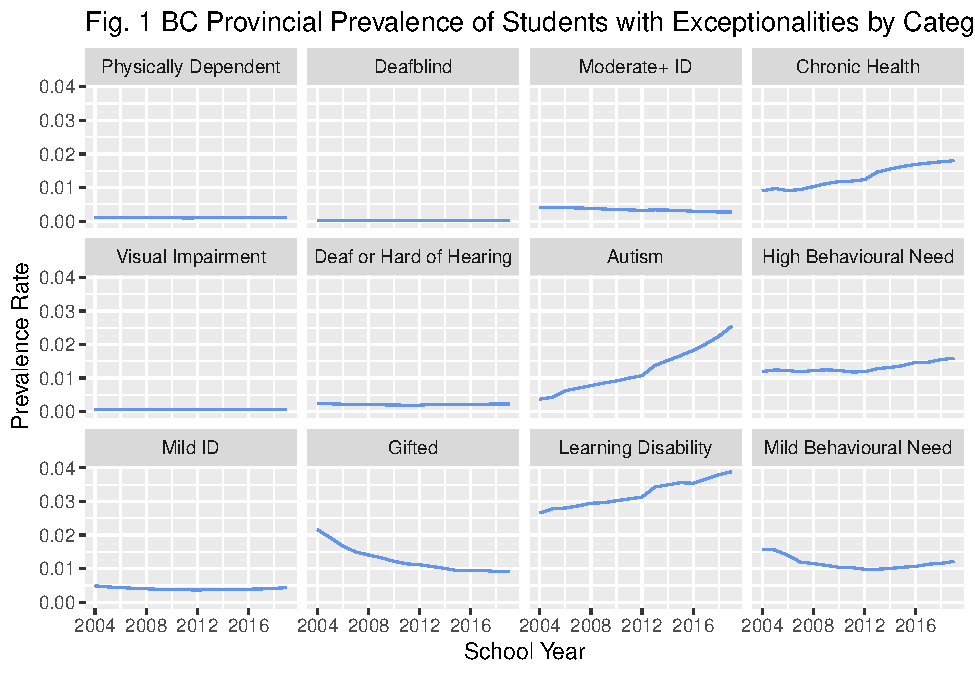
\includegraphics{Final_project_files/figure-latex/Provinical_Data_Overview-1.pdf}

\begin{verbatim}
## # A tibble: 198 x 18
##    year  disability    x6    x7    x8    x9   x10   x11   x12   x13   x14   x15
##    <chr> <chr>      <dbl> <dbl> <dbl> <dbl> <dbl> <dbl> <dbl> <dbl> <dbl> <dbl>
##  1 2002~ INTELLECT~   135   172   220   261   279   303   370   364   388   378
##  2 2002~ HEARING I~    46    66    69    67    79    78    69    70    53    72
##  3 2002~ SPEECH OR~  2502  2466  2443  2205  1894  1282   874   677   493   340
##  4 2002~ VISUAL IM~    18    27    25    16    12    26    19    24    31    19
##  5 2002~ EMOTIONAL~    81   178   241   292   347   433   504   487   549   548
##  6 2002~ ORTHOPEDI~    65    77    64    49    64    71    50    48    44    43
##  7 2002~ DEAF-BLIN~     0     2     0     0     1     0     2     0     4     2
##  8 2002~ MULTIPLE ~     0     0     0     0     0     0     0     0     0     0
##  9 2002~ AUTISM       267   289   290   334   325   316   290   256   243   219
## 10 2002~ TRAUMATIC~     6    11    17    23    22    19    21    23    36    36
## # ... with 188 more rows, and 6 more variables: x16 <dbl>, x17 <dbl>,
## #   x18 <dbl>, x19 <dbl>, x20 <dbl>, x21 <dbl>
\end{verbatim}

\begin{verbatim}
## # A tibble: 198 x 3
## # Groups:   year [18]
##     year disability                    total
##    <dbl> <chr>                         <dbl>
##  1  2002 AUTISM                         3339
##  2  2002 DEAF-BLINDNESS                   17
##  3  2002 DEVELOPMENTAL DELAY               0
##  4  2002 EMOTIONAL DISTURBANCE          4736
##  5  2002 HEARING IMPAIRMENT              873
##  6  2002 INTELLECTUAL DISABILITY        4387
##  7  2002 MULTIPLE DISABILITIES             0
##  8  2002 ORTHOPEDIC IMPAIRMENT           754
##  9  2002 SPEECH OR LANGUAGE IMPAIRMENT 15784
## 10  2002 TRAUMATIC BRAIN INJURY          306
## # ... with 188 more rows
\end{verbatim}

This is roughly in line with Oregon's designation data, showing that there were no state-wide anomalies after the year 2016.

\begin{verbatim}
## Warning: Removed 190 rows containing non-finite values (stat_smooth).
\end{verbatim}

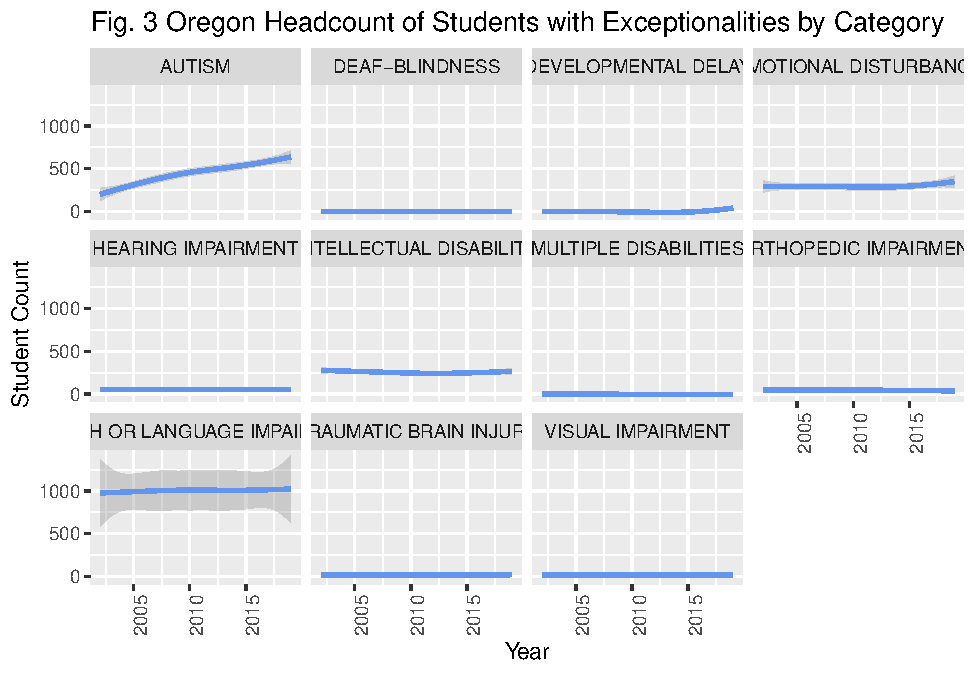
\includegraphics{Final_project_files/figure-latex/unnamed-chunk-1-1.pdf}

Even for diagnostically malleable categories, such as students classified in Oregon has having an \enquote{emotional disturbance,} or in BC students requiring a \enquote{high behavioural need}, Oregon and BC had highly similar trends.

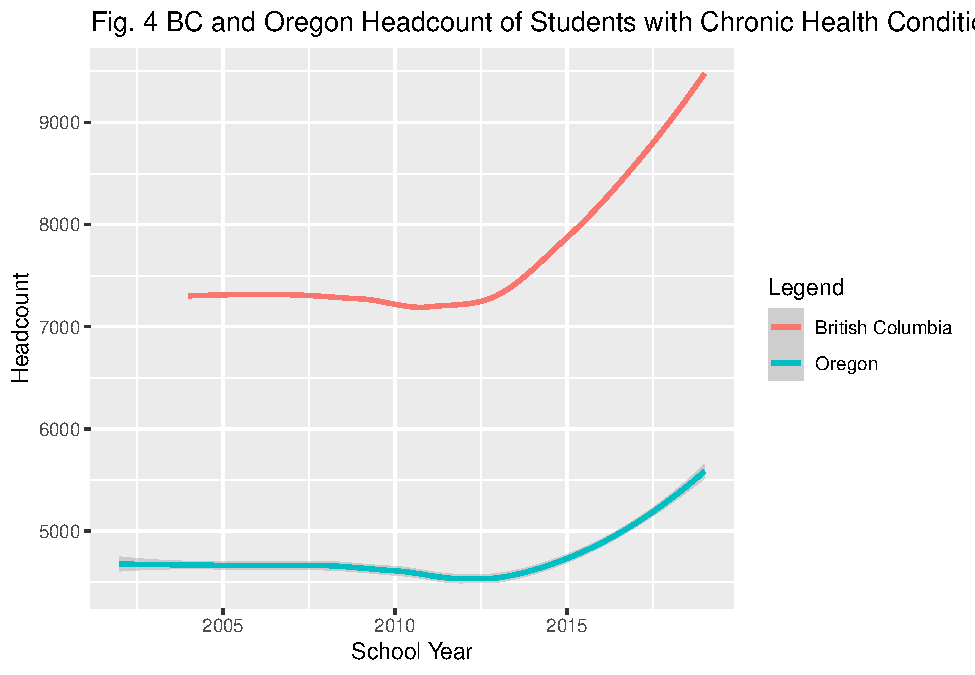
\includegraphics{Final_project_files/figure-latex/BCOR combo-1.pdf}

Then, we examine the rural versus urban trends and notice a few things\ldots{}

\begin{verbatim}
## Warning in FUN(newX[, i], ...): NAs introduced by coercion
\end{verbatim}

\begin{table}[tbp]

\begin{center}
\begin{threeparttable}

\caption{\label{tab:District Census Population Table}District Classification by Population According to 2016 Census}

\begin{tabular}{lllll}
\toprule
District Number & District Name & Population & Classification & Number of Students\\
\midrule
022 & Vernon & 61,334 & Rural & 16,768\\
023 & Central Okanagan & 194,882 & Urban & 43,609\\
028 & Quesnel & 23,146 & Rural & 9,036\\
033 & Chilliwack & 101,512 & Urban & 28,997\\
034 & Abbotsford & 180,518 & Urban & 38,369\\
035 & Langley & 2,463,431 & Urban & 43,043\\
036 & Surrey & 2,463,431 & Urban & 143,222\\
037 & Delta & 2,463,431 & Urban & 43,897\\
038 & Richmond & 2,463,431 & Urban & 40,221\\
039 & Vancouver & 2,463,431 & Urban & 132,584\\
040 & New Westminster & 2,463,431 & Urban & 11,714\\
041 & Burnaby & 2,463,431 & Urban & 47,952\\
042 & Maple Ridge-Pitt Meadows & 2,463,431 & Urban & 33,633\\
043 & Coquitlam & 2,463,431 & Urban & 88,291\\
044 & North Vancouver & 2,463,431 & Urban & 39,657\\
045 & West Vancouver & 2,463,431 & Urban & 11,732\\
046 & Sunshine Coast & 2,463,431 & Urban & 13,283\\
047 & Powell River & 16,783 & Rural & 6,816\\
052 & Prince Rupert & 12,687 & Rural & 7,222\\
053 & Okanagan Similkameen & 43,432 & Rural & 6,596\\
057 & Prince George & 86,622 & Rural & 39,443\\
061 & Greater Victoria & 367,770 & Urban & 50,051\\
062 & Sooke & 367,770 & Urban & 24,126\\
063 & Saanich & 367,770 & Urban & 19,533\\
067 & Okanagan Skaha & 43,432 & Rural & 19,156\\
068 & Nanaimo-Ladysmith & 104,936 & Urban & 30,870\\
070 & Port Alberni & 25,112 & Rural & 11,654\\
073 & Kamloops-Thompson & 103,811 & Urban & 32,620\\
075 & Mission & 33,261 & Rural & 13,858\\
079 & Cowichan Valley & 44,451 & Rural & 21,479\\
081 & Fort Nelson & 18,307 & Rural & 1,319\\
083 & North Okanagan-Shuswap & 43,432 & Rural & 23,720\\
\bottomrule
\addlinespace
\end{tabular}

\begin{tablenotes}[para]
\normalsize{\textit{Note.} Number of students is estimated and does not include masked data.}
\end{tablenotes}

\end{threeparttable}
\end{center}

\end{table}

\begin{verbatim}
## Warning: Removed 129 row(s) containing missing values (geom_path).
\end{verbatim}

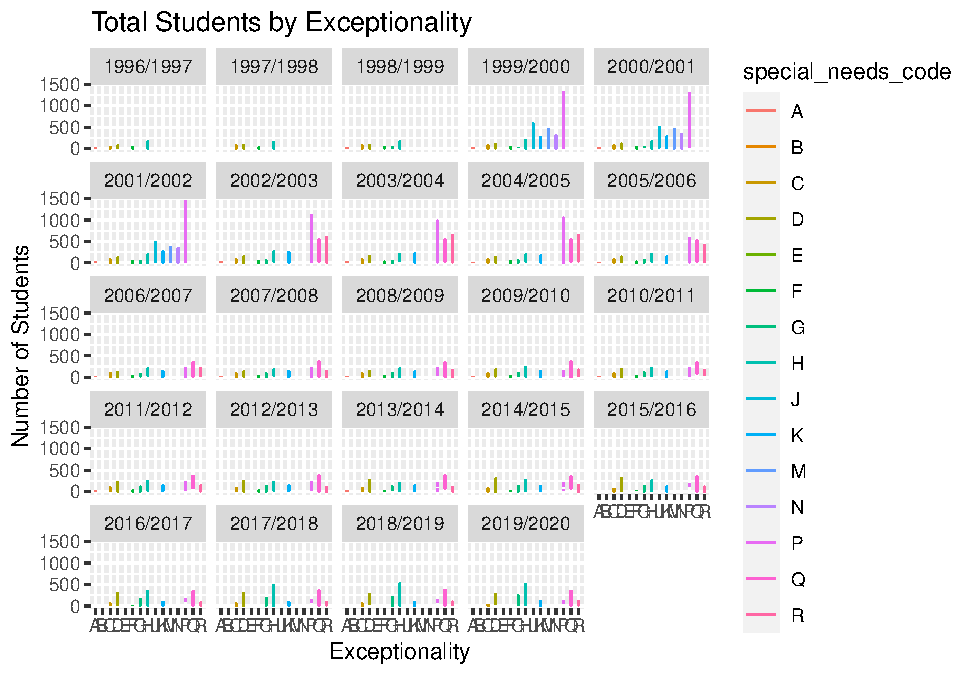
\includegraphics{Final_project_files/figure-latex/rural play-1.pdf} 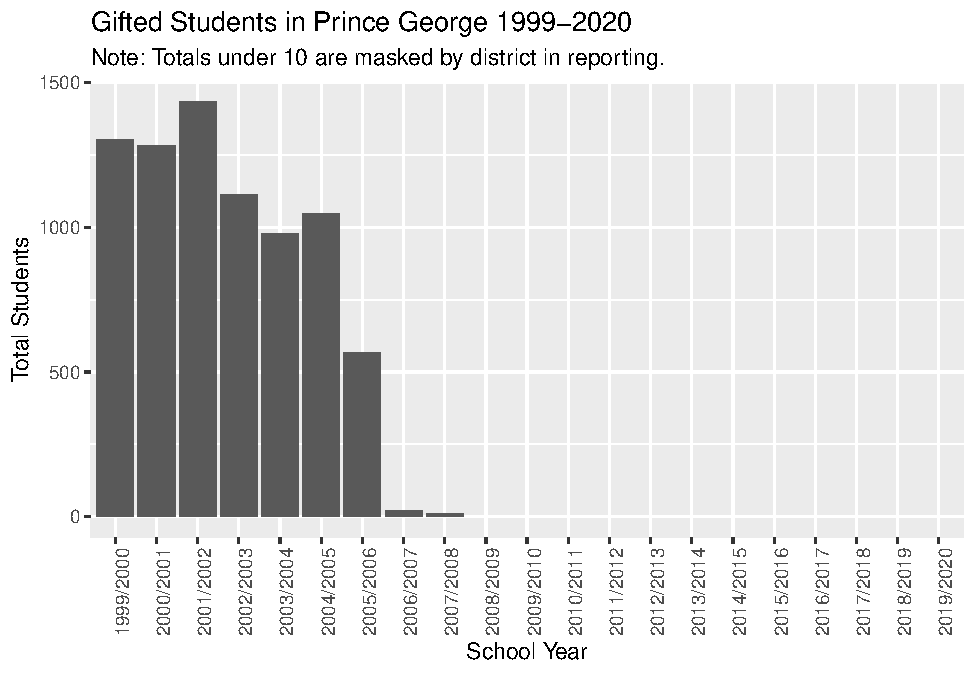
\includegraphics{Final_project_files/figure-latex/rural play-2.pdf} 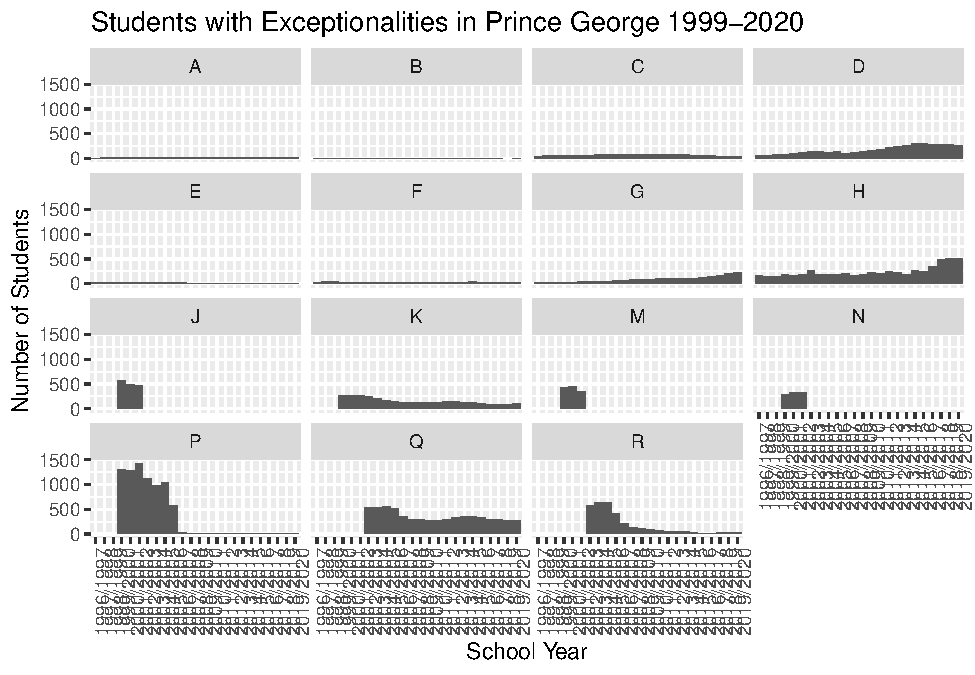
\includegraphics{Final_project_files/figure-latex/rural play-3.pdf}

\begin{verbatim}
## Warning: Removed 12 rows containing missing values (position_stack).
\end{verbatim}

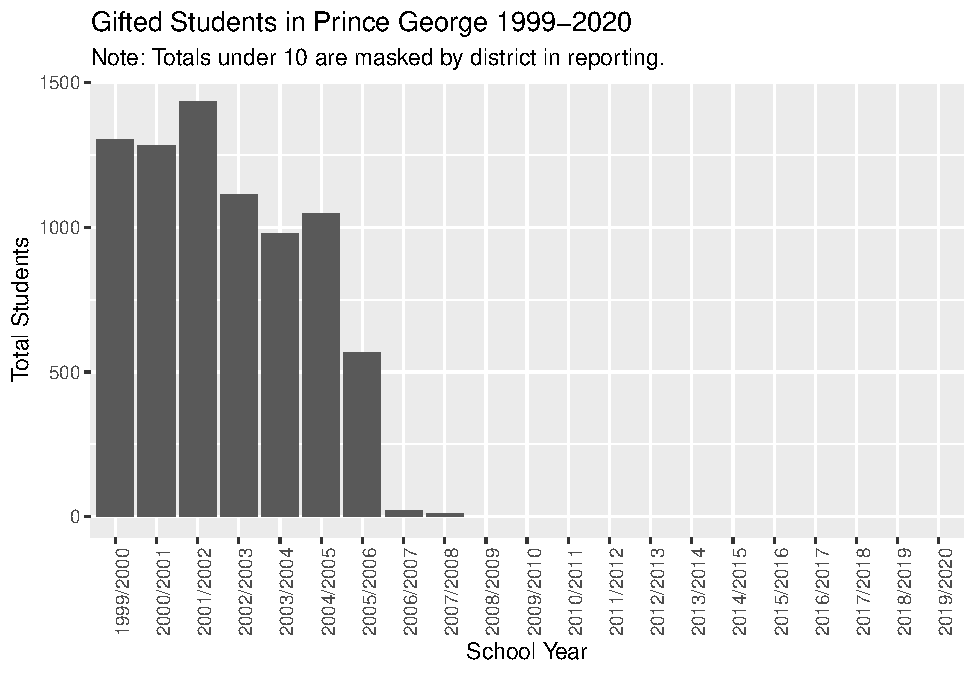
\includegraphics{Final_project_files/figure-latex/rural play-4.pdf} 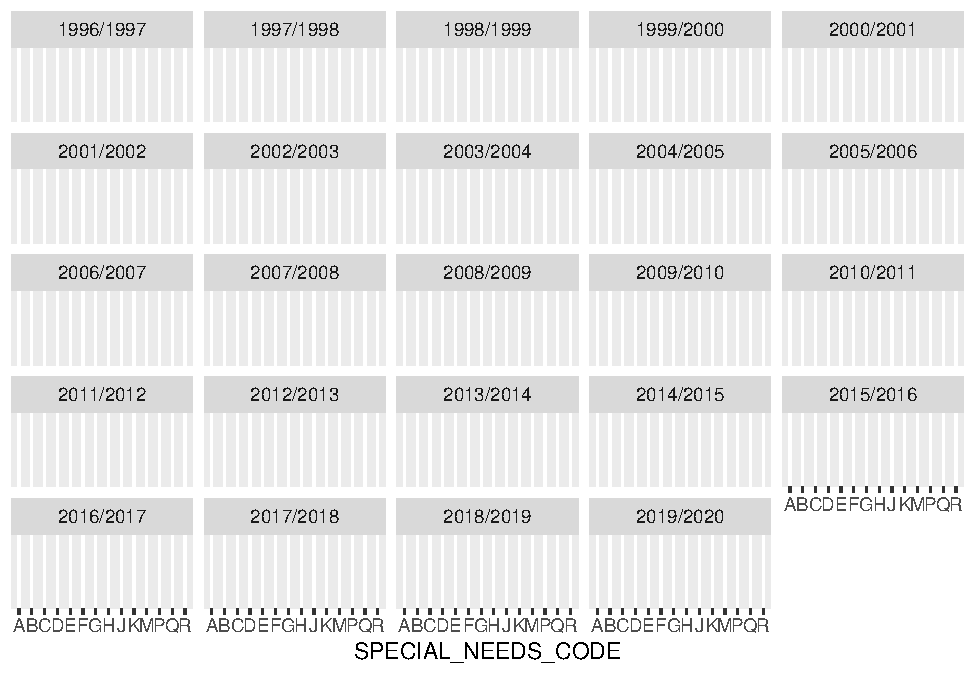
\includegraphics{Final_project_files/figure-latex/rural play-5.pdf}

\begin{verbatim}
## geom_col: width = NULL, na.rm = FALSE
## stat_identity: na.rm = FALSE
## position_stack
\end{verbatim}

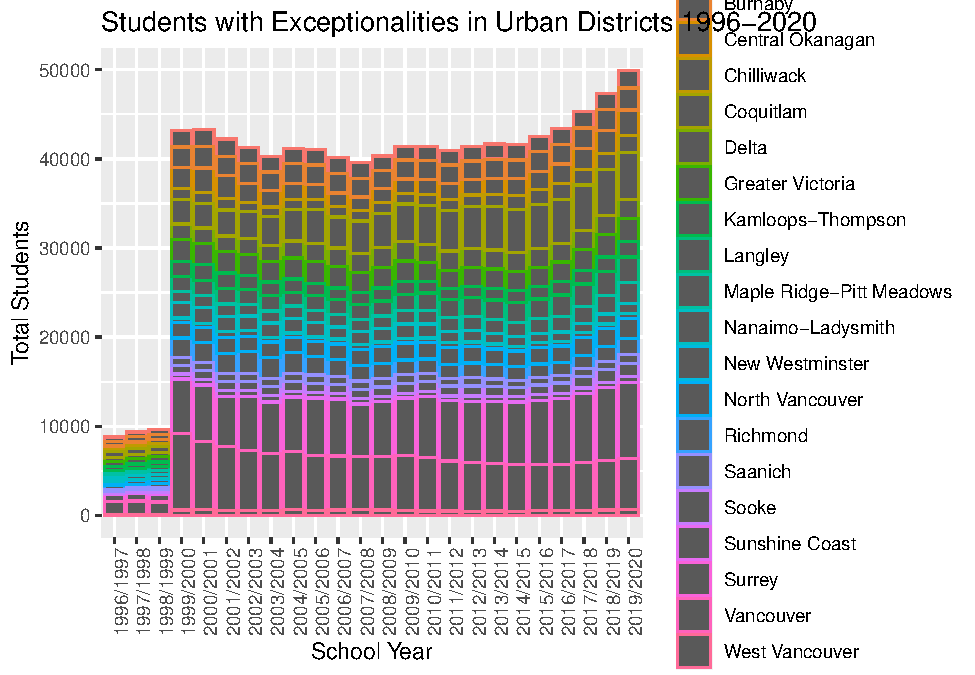
\includegraphics{Final_project_files/figure-latex/urban play-1.pdf}

\begin{verbatim}
## Warning: Removed 25 row(s) containing missing values (geom_path).
\end{verbatim}

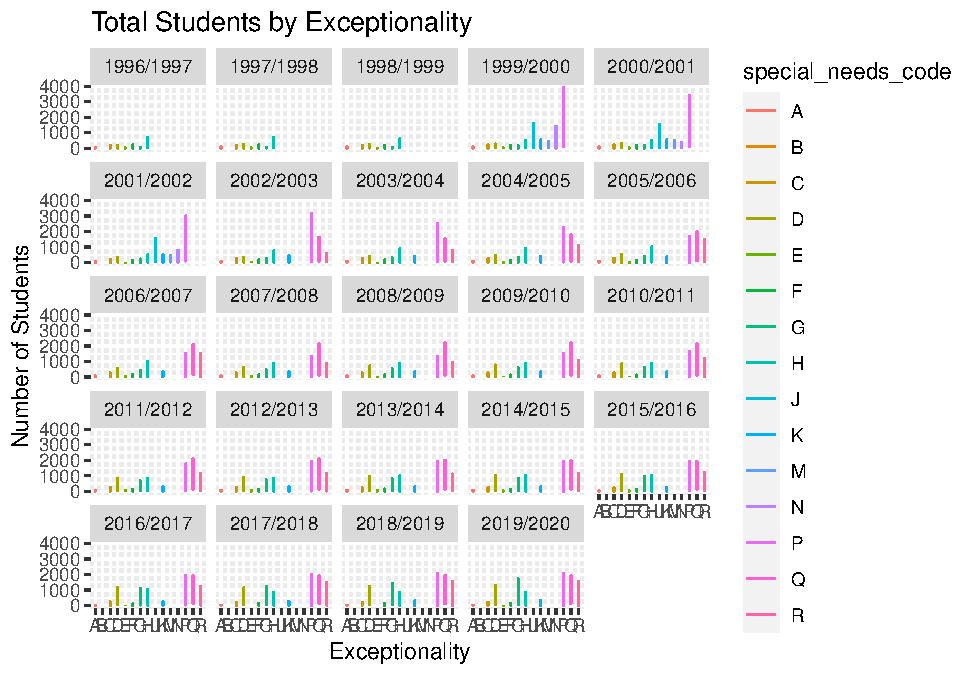
\includegraphics{Final_project_files/figure-latex/urban play-2.pdf}

\hypertarget{discussion}{%
\section{Discussion}\label{discussion}}

Regarding the first research question, it is apparent that the 2016 supreme court decision did not impact any of the 12 designation categories as hypothesized. The trendlines for each of the exceptionality categories remained consistent post-2016 in BC and this mapped on to Oregon trends in exceptionality designation reasonably closely. This finding suggests that the resources and practices around supporting student

The rapid decrease in students identified as gifted in rural districts between the years of 2004 and 2007 cannot be explained by one sole factor in this exploratory analysis. With respect to the speculative nature of this assertion, the authors assume that educational policy at the provincial level impacts educational practice across school districts. In 2006, the British Columbia Ministry of Education released Special education services: A manual of policies, procedures and guidelines, which explicitly states the acceleration programming that should be afforded to students with exceptional academic talent (Kanevsky \& Clelland, 2016). In fact, this 2006 version of the manual was a revision of the original 1995 manual, and this initial version included scant guidance on service provision to gifted students. This 2016 shift in policy links to a higher degree of resources afforded to gifted students through \enquote{independent, guided education} (p.~52). Given the additional resources needed to properly implement gifted educational services, rural school districts may have de-designated students and sought other ways to provide instruction that meets the needs of their students. For example, Lo et al.~(2019) suggest that the British Columbia Ministry of Education's recent curriculum update makes amends for traditional test-and-place gifted student support model by giving educators the tools and inclusive framework to offer a rich, meaningful education to all students with exceptionalities.


\end{document}
